\section{Durchführung}
\label{sec:Durchführung}
Der Aufbau, dargestellt in Abbildung \ref{fig:Aufbau}, besteht aus einer optischen Bank, auf der eine Halogenlampe und beweglicher Schirm befestigt wird. 
Zwischen diesen wird ein Gegenstand installiert welcher im Folgenden auch als 'Pearl L' bezeichnet wird.
Es befindet sich bei der Position $P_G=\qty{25(0.1)}{\centi\meter}$ und besitzt die Größe $G=\qty{3(0.1)}{\centi\meter}$.


\begin{figure}[H]
    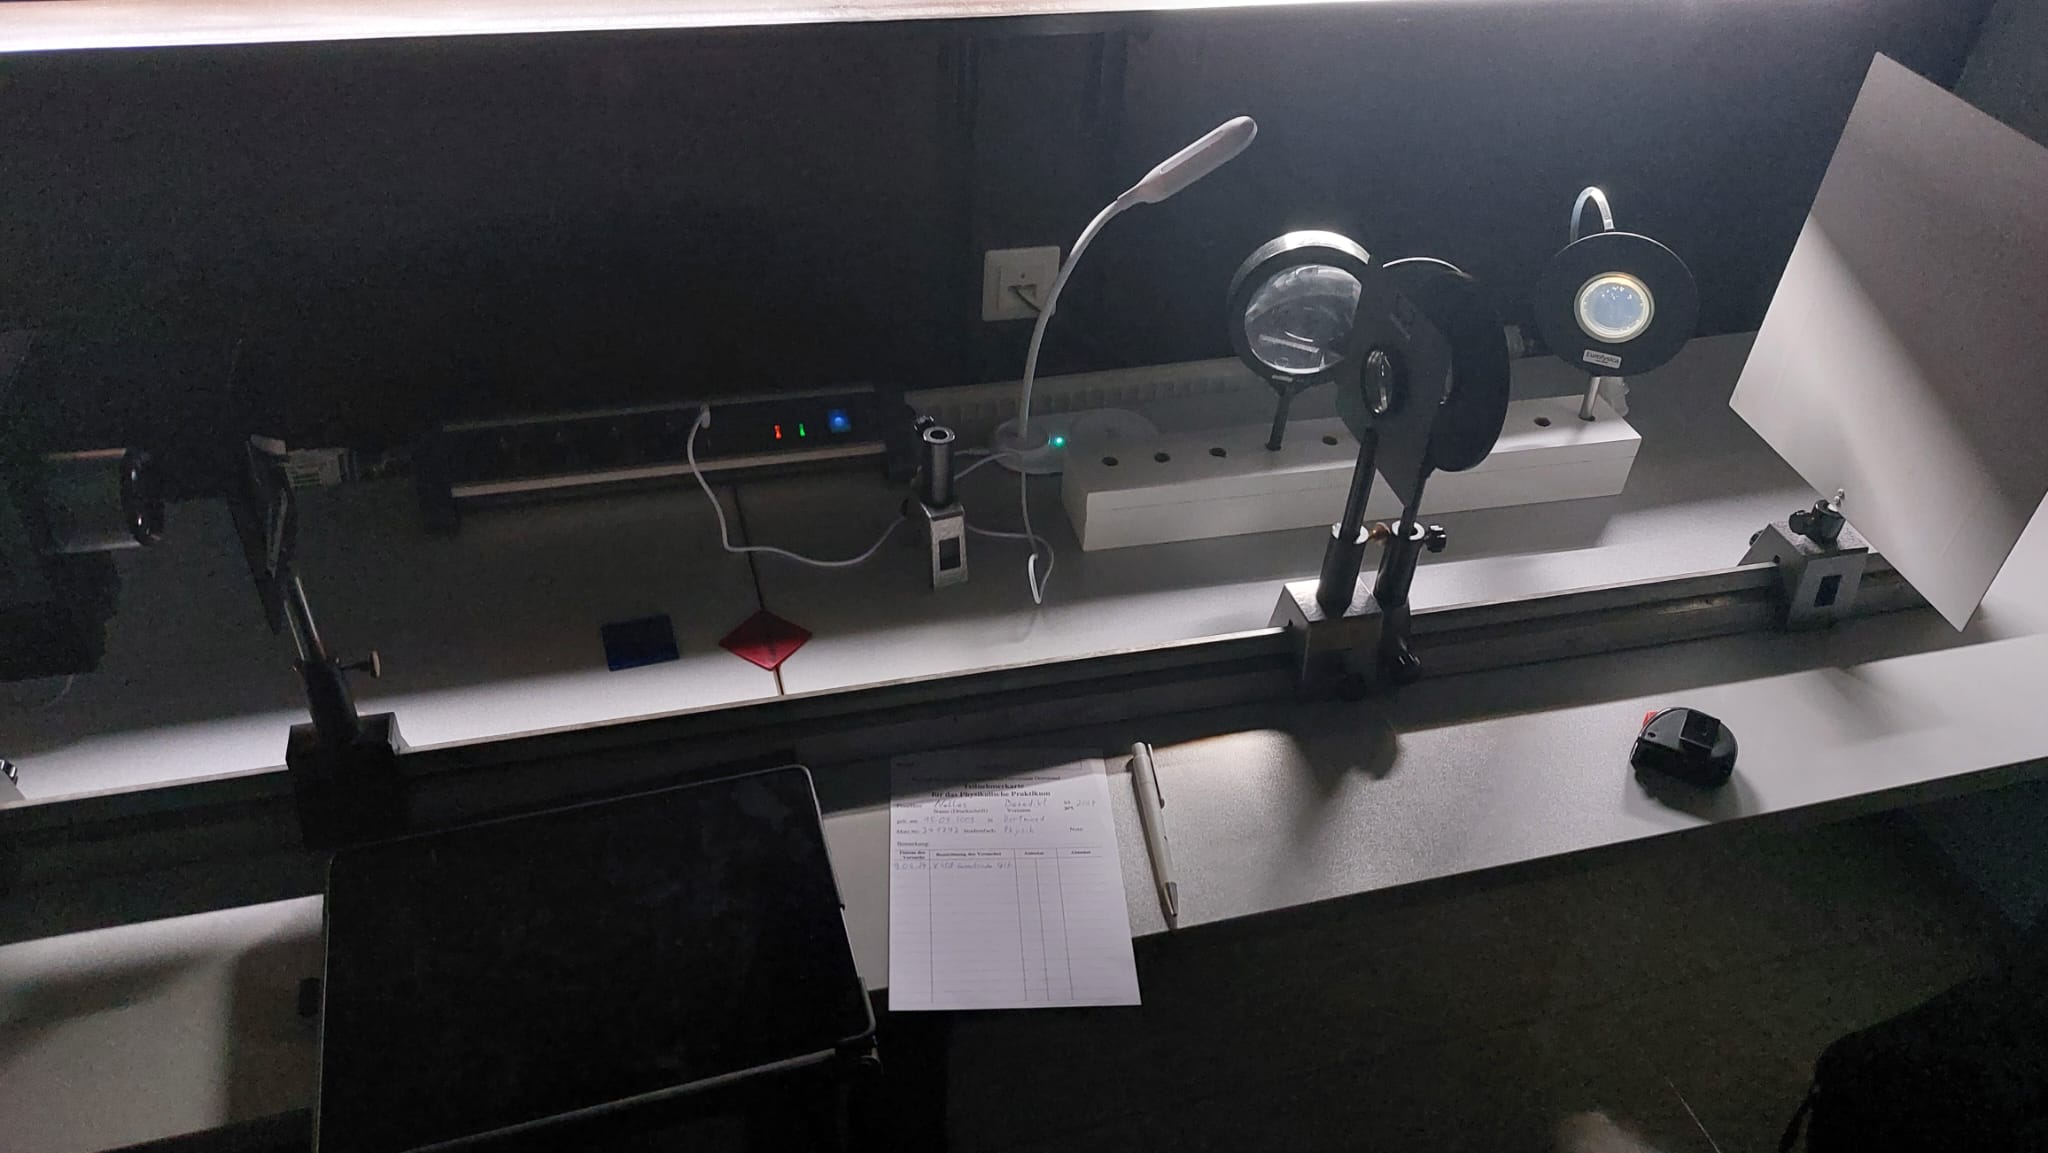
\includegraphics[width=\textwidth]{Bilder/Aufbau.jpg}
    \centering
    \caption{Zu sehen ist der Aufbau des Versuches, links befindet sich die Halogenlampe und der Gegenstand, rechts die Sammellinse und der Schirm.}
    \label{fig:Aufbau}
\end{figure}

\subsection{Bestimmung der Brennweite}
Eine Sammellinse bekannter Brennweite, in diesem Fall $\qty{100}{\milli\meter}$, wird zwischen Gegenstand und Schirm aufgestellt.
Für diese werden 10 Messwerte der Position des Schirms bei verschiedenen Positionen der Linse aufgenommen, wobei der Schirm so lange verschoben wird, bis das Bild scharf zu sehen ist.
Dabei werden auch Werte für die Größe des Bildes aufgenommen, welche mithilfe eines Maßbandes abgelesen werden.

\subsection{Methode von Bessel}
Für eine feste Position des Schirmes wird hier die Linse so lange verschoben, bis ein scharfes Bild erkennbar ist. 
Danach wird dieses weiter in Richtung Schirm geschoben, bis zum zweiten Mal ein scharfes Bild auftaucht.
Die Position der Linse ist in Abbildung \ref{fig:Bessel} erkennbar.
Beide Positionen der Linse so wie die des Schirmes werden für 10 Abstände zwischen Lampe und Schirm gemessen.
Daraufhin wird erst eine blaue und dann eine Rote durchsichtige Platte hinter die 'Pearl L' gesetzt um die Messung für jeweils 5 Abstände wiederholt.
Damit soll die chromatische Aberration überprüft werden.

\begin{figure}[H]
    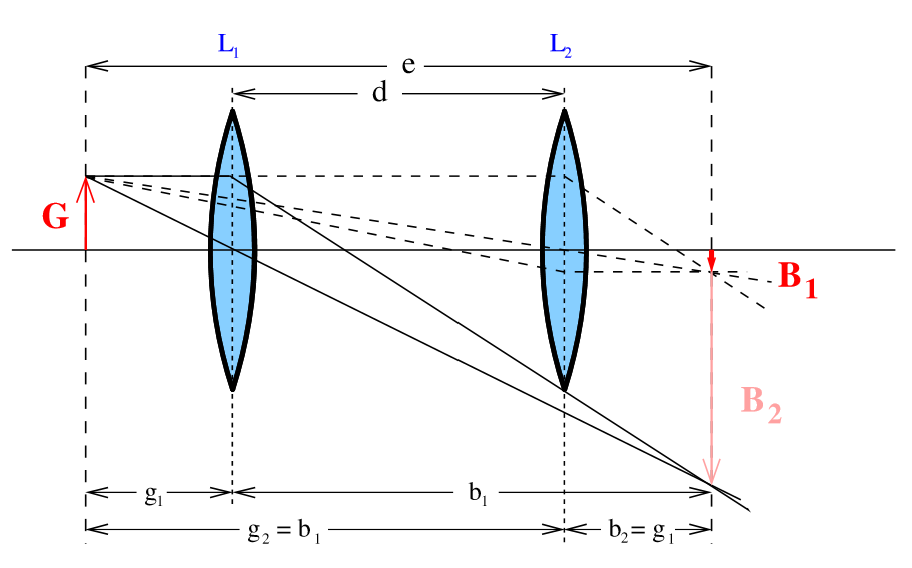
\includegraphics{Bilder/Bessel.png}
    \centering
    \caption{Hier ist schematisch die Position der Linsen bei der Methode von Bessel zur Bestimmung der Brennweite einer Linse dargestellt \cite{V408}.}
    \label{fig:Bessel}
\end{figure}


\subsection{Methode von Abbe}
Vor die Sammellinse wird eine Streulinse mit ebenfalls $\qty{100}{\milli\meter}$ wie in Abbildung \ref{fig:Abbe} installiert.
Die Linsen werden zusammengestellt und bleiben auch zusammen für den weiteren Verlauf des Versuches.
Hierbei wird der Referenzpunkt der Linsen festgesetzt und der Schirm so lange nach hinten verschoben, bis ein scharfes Bild erkennbar wird.
Mit der Kante des Linsenreiters zwischen den Linsen als Referenzpunkt $\symup{A}$ werden 10 Messungen der Position des Referenzpunktes für verschiedene Gegenstandsweiten durchgeführt.


\begin{figure}[H]
    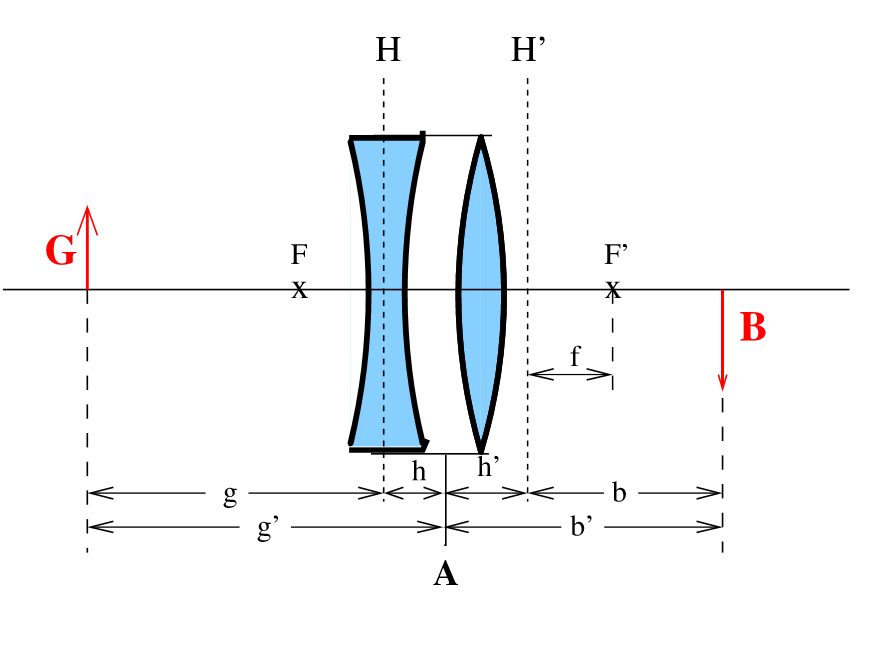
\includegraphics{Bilder/Abbe.png}
    \centering
    \caption{Abgebildet ist hier der Aufbau der Methode von Abbe \cite{V408}.}
    \label{fig:Abbe}
\end{figure}
